\chapter{Implementation Design}
\label{chaptImplementation}
In this chapter, we will introduce the implementation of our demo game and explain the basic principles and algorithms behind it.
\todo {mention measurements}

After consideration of the various approaches implemented in games and also proposed efficient solutions to the problem of real-time destructible environment, we decided to implement and test a combination of reviewed techniques.  

At first, we considered implementation based on \emph{A fast method for simulating destruction and the generated dust and debris} (see \cref{sec:edem}). However, after degrading performance issues~\cref{sec:testing} we decided to abandon this approach.

Our approach is similar to \emph{Geomod} (described in \cref{sec:common}) and \emph{Real Time Dynamic Fracture with Volumetric Approximate Convex Decompositions}(RTDF) (described in \cref{sec:RTDF}), but with several key differences described below. 

\section{Main algorithm}
As mentioned, our algorithm will use boolean operations similarly to \emph{Geomod}, but applied to rigid body objects. The shape of removed object will be determined by Voronoi cell that will be generated dynamically for every collision. The collision information is received from the physics engine.

Our approach generates Voronoi cell at the point of collision. Then the difference of original mesh and the Voronoi cell is calculated and represents the damaged object. To generate the debris, the intersection of original mesh and the Voronoi cell is calculated. This action effectively cuts the object into two or more pieces, all of which are put back into simulation and can be damaged again (see \cref{fig:subtraction}). The Voronoi cell was chosen because it has easily randomizable shape and provides aesthetically good results. This choice is in no way critical to the rest of algorithm, and any other closed mesh can be used as well.

Similarly to the RTDF approach, the cost of fracturing in our implementation is solely dependent on the size and complexity of the fractured object. \todo{odkaz na merania} This makes the method suitable for use in computer games with a large number of simple objects with low polygon meshes.

\begin{figure}
        \centering
        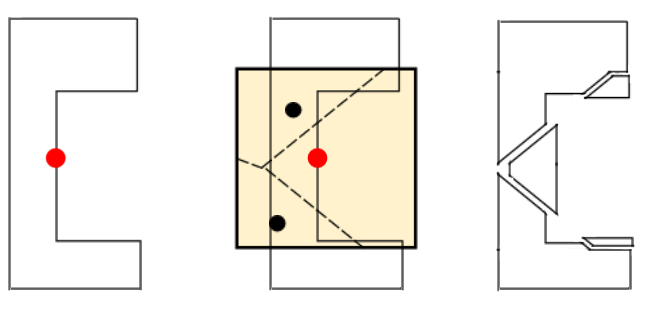
\includegraphics[width=\textwidth]{img/subtractionProcess}
        \caption{object with point of collision (left), generated Voronoi cells (centre), object divided into five new smaller objects after subtraction of the Voronoi cell belonging to the point of collision (right)}
        \label{fig:subtraction}
\end{figure}

To generate the Voronoi cell, we create a closed domain with the centre at the point of collision. In the domain, we need to create random points for generation of their Voronoi cells, and we also add the point of collision. Now we can use a Voronoi cell belonging to the point of collision as the object we subtract from the object in the collision. The boundaries of the domain clip the generated Voronoi cell, therefore the Voronoi cell can never be larger than the domain. Randomization of the size and shape of a Voronoi cell guarantees different result after every collision.

\section{Program Structure}
The main program loop runs in following steps:
\begin{enumerate}
\item Perform a step in physics simulation.
\item Handle collisions and perform destruction, see \cref{sec:collisions}.
\item Read user input and then apply correct forces to controlled vehicle.
\item Render current state of objects. In this step, a graphical representation of every object is updated to comply with its rigid body version.
\end{enumerate}

\begin{figure}
        \centering
        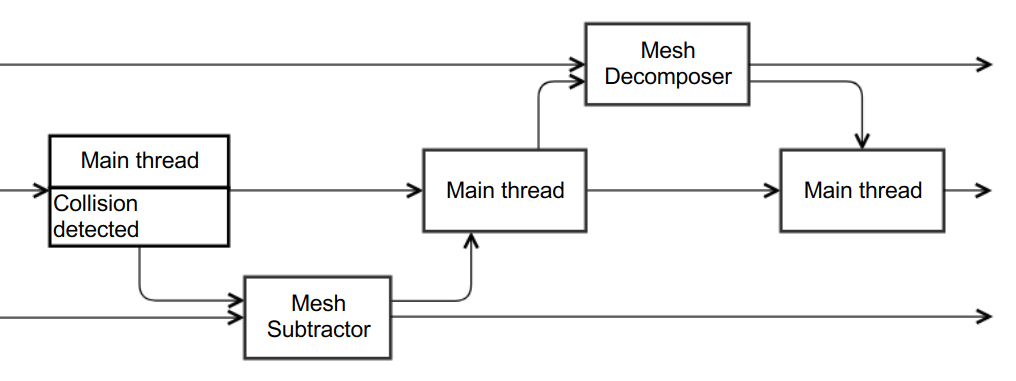
\includegraphics[width=\textwidth]{img/decompositionFlow}
        \caption{Diagram is showing multiple threads handling collision event. }
        \label{fig:threads}
\end{figure}
To make the simulation faster, we execute the most costly tasks asynchronously in separate threads. These tasks are convex decomposition and mesh subtraction. As a result, the program is running in three threads (\cref{fig:threads}): the main thread, a thread for subtracting meshes and a thread for decomposing triangular mesh into a set of convex shapes (\cref{sec:decomposition}). Both subtraction and decomposition threads communicate solely with the main thread, and all communication is done in producer-consumer model. Figure \ref{fig:objectInThreads} shows the changes of the object and its collision shape across all threads.

We use only one thread for all mesh subtraction tasks because we anticipate that the most of the consecutive collisions are going to be triggered by the same object --- shooting at one building multiple times in a row. In this situation, one subtraction does not have valid input data until the previous one has finished, which leads to sequential processing.

A use of a larger thread pool could be useful for convex decomposition. The conflicting state in a decomposition means that the object has changed since our calculation started and a new decomposition task was created. We do not know whether the newer task has already finished or not, but we know for certain, that if we discard our decomposition, the object has either temporary shape or a new valid decomposition. We did not implement a thread pool solution because we did not see it necessary and our hardware was not well suited for running more than four simultaneous threads.

\begin{figure}
        \centering
        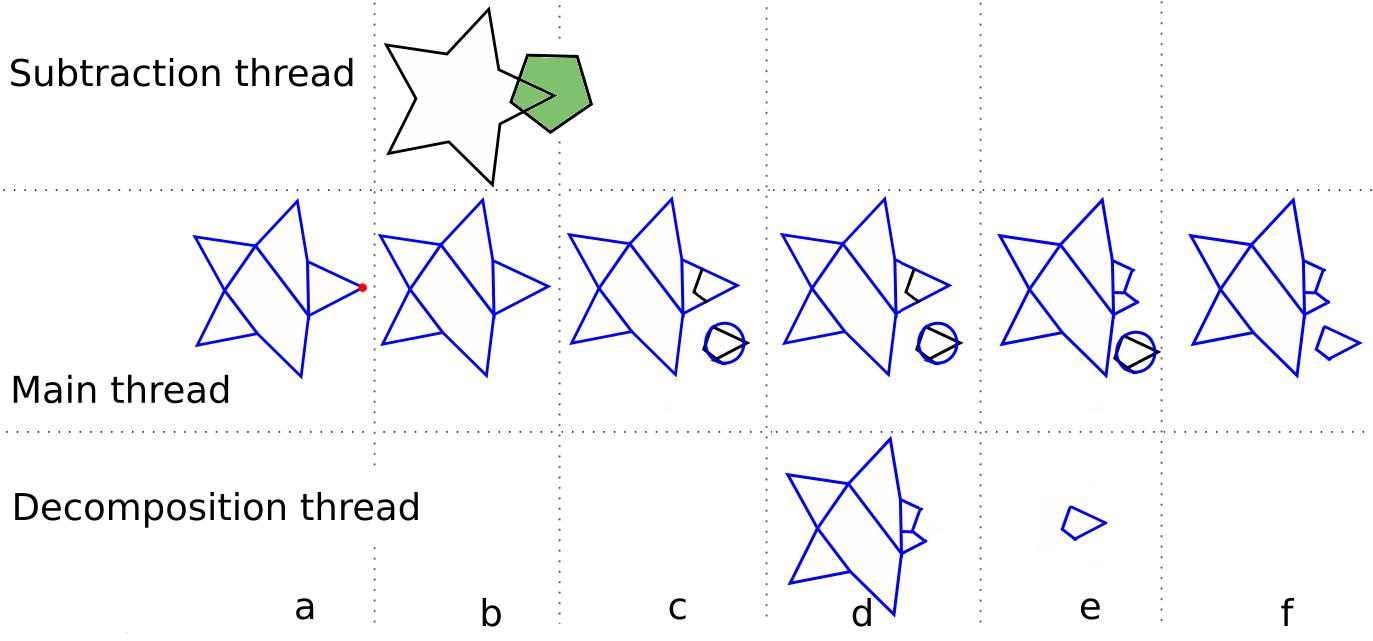
\includegraphics[width=\textwidth]{img/object-progress}
        \caption{Simplified overview of changing states of a single object across multiple threads in simultaneous time slots. We can see the process of splitting the mesh and calculation of collision shapes from the time of the collision until the convex decomposition is calculated for all parts. Blue lines represent the collision shape. Black lines represent the visual mesh (not shown if it is the same as the collision shape), red dot represents the collision point.}
        \label{fig:objectInThreads}
\end{figure}

\section{Collision handling}
\label{sec:collisions}
\todo{odkud se vemou ty reference?}
After the collision, we get a reference to two rigid bodies participating in the collision, point of collision and vector of force from the physics engine. For simplification, we will consider only one object, the point of impact and the force.

At first, we need to filter out unwanted collisions (collisions that should not damage the object). Those collisions can be results of an object placed on ground or collisions with not enough force to damage the object. 

For every valid\todo{`valid' znamena `not unwanted' z predchoziho odstavce?} collision, we generate Voronoi cell as described before, and put \todo{move?} meshes of both objects into a task for mesh subtraction thread. After enqueuing all collisions, we can check if there are any prepared subtraction results for further use. The result of one subtraction task is a set of meshes that represent new objects. For every mesh, we create a new object, but we do not have its convex decomposition for the physics engine to perform accurate collision detection. Because the decomposition can take relatively long, we create a simple temporary collision shape (\eg sphere) and a task for decomposition\todo{of the sphere?}. Then we proceed with simulation, not waiting for the result. Decomposition is done in a separate thread, and the result is returned to the main thread where we check for decomposed shapes. With the shape ready in the main thread we replace the temporary shape for compound shape consisting of convex parts.

This process guarantees that we do not wait for either subtraction or decomposition and therefore we can have stable fps in our game. Temporarily replacing a collision shape by a simpler alternative ensures consistent behaviour of new objects (we can put them into the simulation, and they do not fall through each other or otherwise not comply with laws of physics)\todo{prvni veta je OK, ale druha uz neni uplne pravda --- kdyz strelis do krychle a chvilku ji nahradis kouli, okoli muze slusne explodovat... To by chtelo bud dovysvetlit presnejc, nebo rict ze ty temporary collision shapes jsou dostatecne podobny (a jak jsi toho docilil). Nasledujici veta by nemela zacinat `Therefore' --- spis neco jako ze nedostatecnej vykon pri pocitani meshu kterej by se jinak podepsal na vykyvech ve FPS jsi nahradil tim ze u slozitejch akci trva dyl nez se projevej.}. Therefore we need to calculate the difference of meshes in a period of a few frames so it can not be seen that it is lagging behind collisions.

\section{Convex Decomposition}
\label{sec:decomposition}
Regardless of used physics engine, our objects are represented as triangular meshes. Implementing mesh to mesh collisions is possible, but highly impractical. Even if checking every vertex of one mesh against all vertices of second mesh is sufficient, the complexity of algorithm would be dependent on the number of vertices. We can imagine a cube made out of eight vertices and the second cube with the same size but subdivided surface into thousands of vertices. Mesh to mesh collision detection algorithm would perform differently on the seamlessly identical objects. This behaviour is not desired in computer games where the surface of the objects is usually subdivided into thousands of triangles to created small details on a mesh.

To be able to perform fast mesh to mesh collisions we must find a way to describe the object as a set of geometrically simpler shapes. The convex shapes are the easiest for detecting mutual intersections, but encapsulating whole mesh into a convex hull would produce imprecise collisions. This problem is solved by performing a convex decomposition. Convex decomposition process splits the input object into a set of convex shapes, forming a compound shape. Now the complexity of the collision algorithm depends on the number of convex parts. 

While the exact convex decomposition can still produce a significant number of convex parts~\cite{convexDecomp}, in the setting of a computer game, the speed of calculation is much more relevant than the precision --- small differences between collision shapes and visual meshes are not considered to be a problem. To be able to perform collision detection at real-time, many approximate convex decomposition algorithms that sacrifice some precision to gain performance have been proposed. One of those algorithms is \emph{Hierarchical Approximate Convex Decomposition} algorithm (see \cref{sec:decompositionLib}) which we decided to use.

\section{Measurements and experiments}
\label{sec:testing}
\todo{nieco rozumne namerat a napisat o tom}

(Napady na mereni, muzes si do programu dodelat hooky ktery ti jen vysypou statistiku a timingy u tech operaci:
\begin{itemize}
\item Kolik prumerne trva prevedeni triangle meshe na HACD --- treba graf co porovnava jakej vliv ma pocet trojuhelniku/konvexnost/konkavnost na dylku vypoctu).
\item Kolik prumerne trva jedno spocitani detekce kolizi v zavislosti na poctu a velikosti objektu?
\item Kolik casu sezere vlakno co dela ten subtraction (zase v zavislosti na tom jak velkej objekt se resi)?
\item Kolik casu sezere vlakno co dela tu dekompozici?
\end{itemize})
\subsection{Testing the concept of EDEM}
To test EDEM (described in \cref{sec:edem}), we set up a cube divided into 439 tetrahedrons. After introducing constraints to hold the tetrahedrons together, we experienced a drop from 60fps (set as an upper limit) to 13fps. Having a large number of elements connected with springs in the simulation can also trigger an undesirable behaviour, such as contractions, retractions and self-induced explosions of the object. Performance issues and problems with keeping elements in a stable state finally concluded that the approach was not suitable for our implementation.

